\documentclass[border=7pt]{standalone}
\usepackage{amsmath,amssymb}
\usepackage{tikz}
\usetikzlibrary{calc,positioning,arrows.meta,shapes.geometric,fit,backgrounds}

% =====================================================================
% Academic Figure Skill — Nature/Cell/Science Semantic Color Palette
% Fig. 2: Online IM-CNN + EMA-VQ & Bisimulation Dynamic Prototype Pool (QA Polished)
% =====================================================================
\definecolor{cBlue}{HTML}{2166AC}
\definecolor{cBlueMid}{HTML}{4393C3}
\definecolor{cBlueLt}{HTML}{92C5DE}
\definecolor{cBluePale}{HTML}{D1E5F0}
\definecolor{cBlueBg}{HTML}{F0F6FC}

\definecolor{cRed}{HTML}{B2182B}
\definecolor{cRedMid}{HTML}{D6604D}
\definecolor{cRedPale}{HTML}{FDDBC7}
\definecolor{cRedBg}{HTML}{FDF2F2}

\definecolor{cGreen}{HTML}{1B7837}
\definecolor{cGreenMid}{HTML}{5AAE61}
\definecolor{cGreenBg}{HTML}{EFF8F1}

\definecolor{cPurple}{HTML}{762A83}
\definecolor{cPurpleMid}{HTML}{9970AB}
\definecolor{cPurpleBg}{HTML}{F7F1FA}

\definecolor{cOrange}{HTML}{B35806}
\definecolor{cOrangeMid}{HTML}{E08214}
\definecolor{cOrangeBg}{HTML}{FEF6EC}

\definecolor{cInk}{HTML}{1E293B}
\definecolor{cMuted}{HTML}{475569}
\definecolor{cGray}{HTML}{94A3B8}
\definecolor{cLine}{HTML}{CBD5E1}
\definecolor{cBand}{HTML}{F1F5F9}
\definecolor{cPanel}{HTML}{F8FAFC}

\newcommand{\tensorblock}[9]{%
  \begin{scope}
    \pgfmathsetmacro{\xL}{#1 - #3/2}
    \pgfmathsetmacro{\xR}{#1 + #3/2}
    \pgfmathsetmacro{\yB}{#2 - #4/2}
    \pgfmathsetmacro{\yT}{#2 + #4/2}
    \pgfmathsetmacro{\dx}{#5 * 0.50}
    \pgfmathsetmacro{\dy}{#5 * 0.38}
    \filldraw[fill=#6, draw=#9, line width=0.6pt, line join=round]
      (\xL,\yB) rectangle (\xR,\yT);
    \filldraw[fill=#7, draw=#9, line width=0.6pt, line join=round]
      (\xL,\yT) -- (\xL+\dx,\yT+\dy) -- (\xR+\dx,\yT+\dy) -- (\xR,\yT) -- cycle;
    \filldraw[fill=#8, draw=#9, line width=0.6pt, line join=round]
      (\xR,\yB) -- (\xR+\dx,\yB+\dy) -- (\xR+\dx,\yT+\dy) -- (\xR,\yT) -- cycle;
  \end{scope}
}

\begin{document}
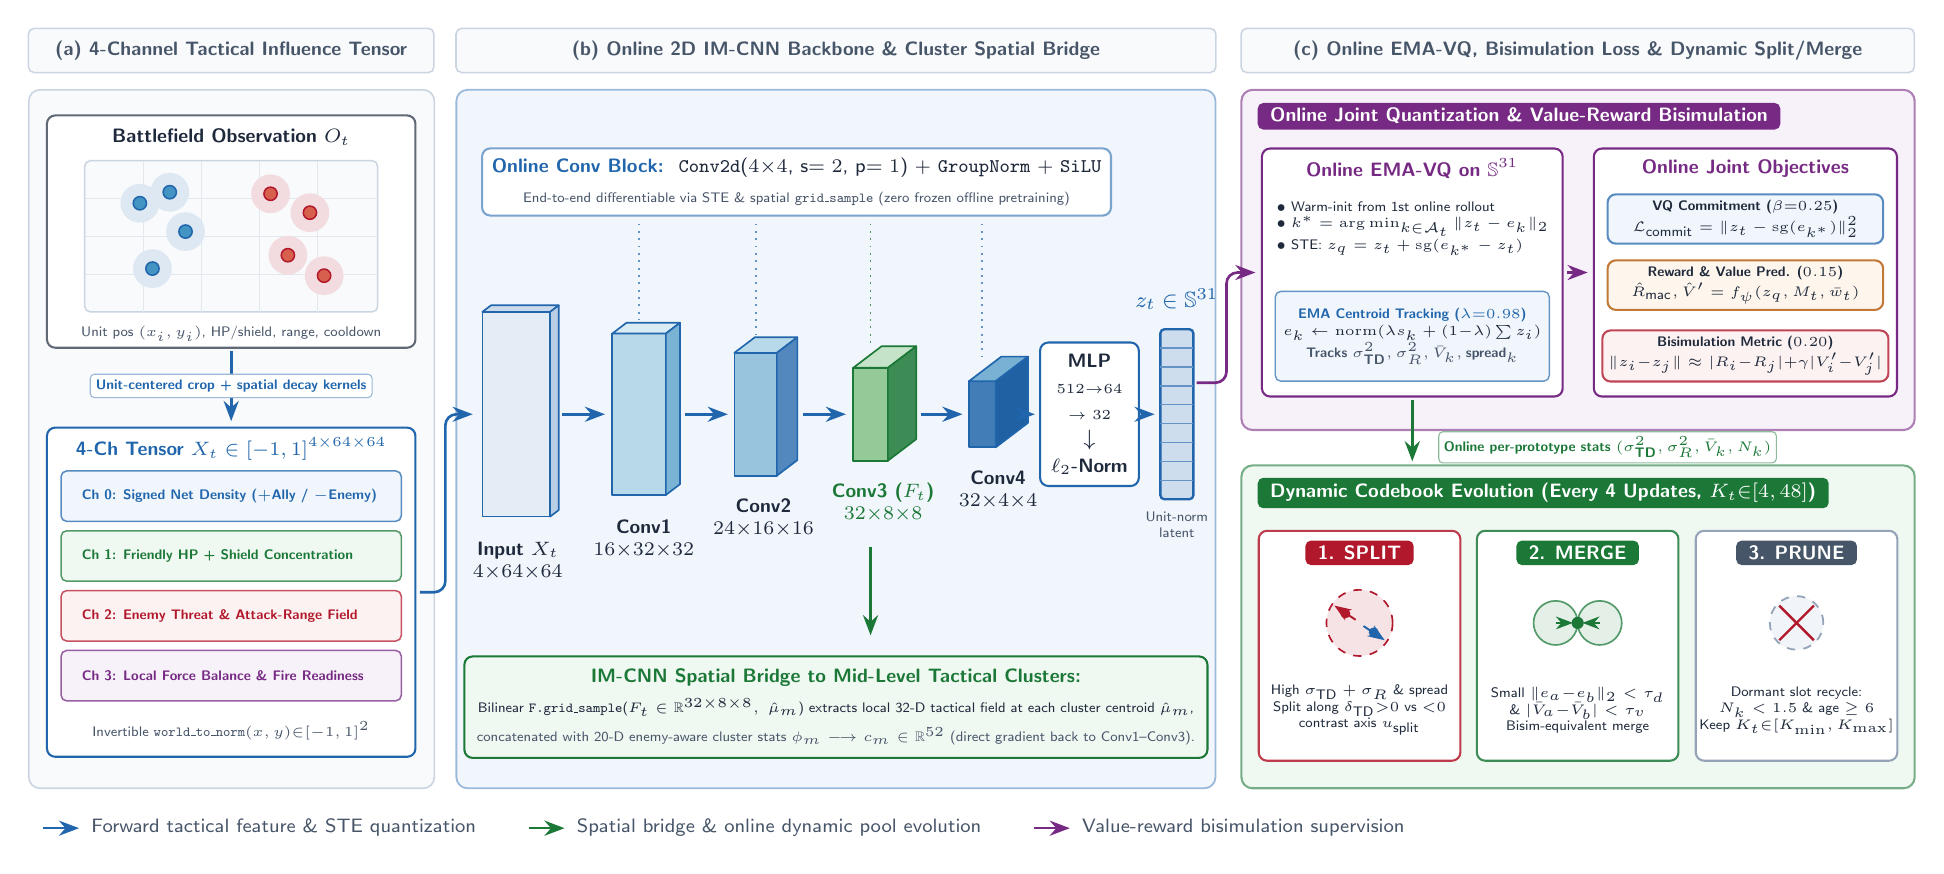
\begin{tikzpicture}[
  x=1cm, y=1cm,
  >=Stealth,
  font=\sffamily\footnotesize,
  box/.style={
    rectangle, rounded corners=3pt, draw=#1, fill=white,
    line width=0.75pt, align=center, inner sep=4pt, text=cInk
  },
  stagehdr/.style={
    rectangle, rounded corners=2pt, fill=cPanel, draw=cLine,
    line width=0.55pt, font=\sffamily\scriptsize\bfseries, text=cMuted,
    minimum height=0.56cm, align=center
  },
  pill/.style={
    rectangle, rounded corners=2pt, fill=#1, text=white,
    font=\sffamily\scriptsize\bfseries, inner xsep=4.5pt, inner ysep=2.0pt
  },
  flow/.style={->, line width=0.95pt, draw=#1, shorten >=1.5pt, shorten <=1.2pt}
]

% 0. Top Banners
\node[stagehdr, minimum width=5.15cm] at (2.62, 10.72) {(a) 4-Channel Tactical Influence Tensor};
\node[stagehdr, minimum width=9.65cm] at (10.30, 10.72) {(b) Online 2D IM-CNN Backbone \& Cluster Spatial Bridge};
\node[stagehdr, minimum width=8.55cm] at (19.72, 10.72) {(c) Online EMA-VQ, Bisimulation Loss \& Dynamic Split/Merge};

% 1. Background Enclosures
\begin{scope}[on background layer]
  \filldraw[fill=cPanel, draw=cLine, rounded corners=4pt, line width=0.6pt]
    (0.05, 1.35) rectangle (5.20, 10.22);
  \filldraw[fill=cBlueBg, draw=cBlue!45, rounded corners=4pt, line width=0.65pt]
    (5.48, 1.35) rectangle (15.12, 10.22);
  \filldraw[fill=cPurpleBg, draw=cPurple!60, rounded corners=4pt, line width=0.75pt]
    (15.45, 5.90) rectangle (24.00, 10.22);
  \filldraw[fill=cGreenBg, draw=cGreen!60, rounded corners=4pt, line width=0.75pt]
    (15.45, 1.35) rectangle (24.00, 5.45);
\end{scope}

\node[pill=cPurple, anchor=north west] at (15.65, 10.06) {Online Joint Quantization \& Value-Reward Bisimulation};
\node[pill=cGreen,  anchor=north west] at (15.65, 5.30) {Dynamic Codebook Evolution (Every 4 Updates, $K_t{\in}[4,48]$)};

% 2. Zone (a)
\node[box=cInk!70, minimum width=4.68cm, minimum height=2.95cm] (ObsCard) at (2.62, 8.42) {};
\node[font=\sffamily\scriptsize\bfseries, text=cInk] at (2.62, 9.62) {Battlefield Observation $O_t$};
\begin{scope}[shift={(0.76, 7.40)}]
  \filldraw[fill=cPanel, draw=cLine, rounded corners=2pt, line width=0.55pt] (0,0) rectangle (3.72, 1.92);
  \foreach \gx in {0.74, 1.48, 2.22, 2.96} {\draw[cLine!55, line width=0.3pt] (\gx,0) -- (\gx,1.92);}
  \foreach \gy in {0.48, 0.96, 1.44} {\draw[cLine!55, line width=0.3pt] (0,\gy) -- (3.72,\gy);}
  \foreach \ux/\uy in {0.70/1.38, 1.08/1.52, 1.28/1.02, 0.86/0.55} {
    \fill[cBlue!15] (\ux,\uy) circle (7pt);
    \filldraw[fill=cBlueMid, draw=cBlue, line width=0.55pt] (\ux,\uy) circle (2.4pt);
  }
  \foreach \ux/\uy in {2.36/1.50, 2.86/1.26, 2.58/0.72, 3.04/0.46} {
    \fill[cRed!15] (\ux,\uy) circle (7pt);
    \filldraw[fill=cRedMid, draw=cRed, line width=0.55pt] (\ux,\uy) circle (2.4pt);
  }
\end{scope}
\node[font=\sffamily\tiny, text=cMuted] at (2.62, 7.12) {Unit pos $(x_i,y_i)$, HP/shield, range, cooldown};

\draw[flow=cBlue] (2.62, 6.94) -- (2.62, 5.96);
\node[font=\sffamily\tiny\bfseries, text=cBlue, fill=white, draw=cBlue!45, rounded corners=1.5pt, inner sep=2pt]
  at (2.62, 6.46) {Unit-centered crop + spatial decay kernels};

\node[box=cBlue, minimum width=4.68cm, minimum height=4.18cm] (IMCard) at (2.62, 3.84) {};
\node[font=\sffamily\scriptsize\bfseries, text=cBlue] at (2.62, 5.66) {4-Ch Tensor $X_t \in [-1,1]^{4\times 64\times 64}$};

\filldraw[fill=cBlueBg,   draw=cBlue!75,   rounded corners=2pt, line width=0.55pt] (0.46, 4.74) rectangle (4.78, 5.38);
\node[font=\sffamily\tiny\bfseries, text=cBlue, anchor=west] at (0.60, 5.06) {Ch 0: Signed Net Density ($+$Ally / $-$Enemy)};

\filldraw[fill=cGreenBg,  draw=cGreen!75,  rounded corners=2pt, line width=0.55pt] (0.46, 3.98) rectangle (4.78, 4.62);
\node[font=\sffamily\tiny\bfseries, text=cGreen, anchor=west] at (0.60, 4.30) {Ch 1: Friendly HP + Shield Concentration};

\filldraw[fill=cRedBg,    draw=cRed!75,    rounded corners=2pt, line width=0.55pt] (0.46, 3.22) rectangle (4.78, 3.86);
\node[font=\sffamily\tiny\bfseries, text=cRed, anchor=west] at (0.60, 3.54) {Ch 2: Enemy Threat \& Attack-Range Field};

\filldraw[fill=cPurpleBg, draw=cPurple!75, rounded corners=2pt, line width=0.55pt] (0.46, 2.46) rectangle (4.78, 3.10);
\node[font=\sffamily\tiny\bfseries, text=cPurple, anchor=west] at (0.60, 2.78) {Ch 3: Local Force Balance \& Fire Readiness};

\node[font=\sffamily\tiny, text=cMuted] at (2.62, 2.08)
  {Invertible \texttt{world\_to\_norm}$(x,y){\in}[-1,1]^2$};

% 3. Zone (b): 3D Isometric Convolutional Feature Pyramid
\draw[flow=cBlue, rounded corners=4pt] (IMCard.east) -- (5.34, 3.84) -- (5.34, 6.10) -- (5.74, 6.10);

\tensorblock{6.24}{6.10}{0.86}{2.60}{0.22}{cBlue!12}{cBlue!24}{cBlue!32}{cBlue}
\node[font=\sffamily\scriptsize\bfseries, text=cInk, align=center] at (6.26, 4.24) {Input $X_t$\\$4{\times}64{\times}64$};

\tensorblock{7.80}{6.10}{0.68}{2.05}{0.36}{cBlueLt!65}{cBlueLt!35}{cBlueMid!70}{cBlue}
\node[font=\sffamily\scriptsize, text=cInk, align=center] at (7.86, 4.52) {\textbf{Conv1}\\$16{\times}32{\times}32$};

\tensorblock{9.28}{6.10}{0.54}{1.56}{0.52}{cBlueMid!55}{cBlueLt!65}{cBlue!78}{cBlue}
\node[font=\sffamily\scriptsize, text=cInk, align=center] at (9.38, 4.78) {\textbf{Conv2}\\$24{\times}16{\times}16$};

\tensorblock{10.74}{6.10}{0.44}{1.18}{0.72}{cGreenMid!65}{cGreenMid!35}{cGreen!85}{cGreen}
\node[font=\sffamily\scriptsize\bfseries, text=cGreen, align=center] at (10.90, 4.98) {Conv3 ($F_t$)\\$32{\times}8{\times}8$};

\tensorblock{12.16}{6.10}{0.34}{0.84}{0.82}{cBlue!85}{cBlueMid!72}{cBlue!95!black}{cBlue}
\node[font=\sffamily\scriptsize, text=cInk, align=center] at (12.36, 5.14) {\textbf{Conv4}\\$32{\times}4{\times}4$};

\draw[flow=cBlue] (6.78, 6.10) -- (7.42, 6.10);
\draw[flow=cBlue] (8.34, 6.10) -- (8.98, 6.10);
\draw[flow=cBlue] (9.84, 6.10) -- (10.48, 6.10);
\draw[flow=cBlue] (11.34, 6.10) -- (11.96, 6.10);

\node[box=cBlue!60, fill=white, minimum width=7.30cm, inner sep=3.5pt] at (9.80, 9.05) {
  {\scriptsize\textbf{\color{cBlue}Online Conv Block:}\; \texttt{Conv2d}($4{\times}4$, s$=2$, p$=1$) + \texttt{GroupNorm} + \texttt{SiLU}}\\[0.15em]
  {\tiny\color{cMuted}End-to-end differentiable via STE \& spatial \texttt{grid\_sample} (zero frozen offline pretraining)}
};
\draw[dotted, cBlue!70, line width=0.65pt] (7.80, 8.52) -- (7.80, 7.30);
\draw[dotted, cBlue!70, line width=0.65pt] (9.28, 8.52) -- (9.28, 7.12);
\draw[dotted, cGreen!80, line width=0.65pt] (10.74, 8.52) -- (10.74, 6.98);
\draw[dotted, cBlue!70, line width=0.65pt] (12.16, 8.52) -- (12.16, 6.84);

\node[box=cBlue, minimum width=1.24cm, minimum height=1.72cm] (FlatFC) at (13.52, 6.10)
  {\scriptsize\textbf{MLP}\\{\tiny $512{\to}64$}\\{\tiny $\to 32$}\\$\downarrow$\\{\scriptsize\textbf{$\ell_2$-Norm}}};
\draw[flow=cBlue] (12.74, 6.10) -- (FlatFC.west);

\filldraw[fill=cBlue!22, draw=cBlue, rounded corners=1.5pt, line width=0.85pt]
  (14.42, 5.02) rectangle (14.84, 7.18);
\foreach \zy in {5.26, 5.50, 5.74, 5.98, 6.22, 6.46, 6.70, 6.94} {
  \draw[cBlue!70, line width=0.45pt] (14.42,\zy) -- (14.84,\zy);
}
\node[font=\sffamily\footnotesize\bfseries, text=cBlue] at (14.63, 7.56) {$z_t \in \mathbb{S}^{31}$};
\node[font=\sffamily\tiny, text=cMuted, align=center] at (14.63, 4.70) {Unit-norm\\latent};
\draw[flow=cBlue] (FlatFC.east) -- (14.40, 6.10);

% Spatial Bridge Box (centered without justified stretch!)
\draw[flow=cGreen] (10.74, 4.46) -- (10.74, 3.24);
\node[box=cGreen, fill=cGreenBg, minimum width=8.95cm, inner sep=4.5pt, align=center] (BridgeBox) at (10.30, 2.38) {
  {\scriptsize\textbf{\color{cGreen}IM-CNN Spatial Bridge to Mid-Level Tactical Clusters:}}\\[0.18em]
  {\tiny\color{cInk}Bilinear \texttt{F.grid\_sample}($F_t \in \mathbb{R}^{32\times 8\times 8},\; \hat{\mu}_m$) extracts local 32-D tactical field at each cluster centroid $\hat{\mu}_m$,}\\[0.12em]
  {\tiny\color{cMuted}concatenated with 20-D enemy-aware cluster stats $\phi_m \longrightarrow c_m \in \mathbb{R}^{52}$ (direct gradient back to Conv1--Conv3).}
};

% 4. Zone (c-top): Online EMA-VQ + Joint Bisimulation Losses
\draw[flow=cPurple, rounded corners=4pt] (14.84, 6.50) -- (15.26, 6.50) -- (15.26, 7.90) -- (15.68, 7.90);

\node[box=cPurple, minimum width=3.82cm, minimum height=3.15cm] (VQBox) at (17.62, 7.90) {};
\node[font=\sffamily\scriptsize\bfseries, text=cPurple] at (17.62, 9.22) {Online EMA-VQ on $\mathbb{S}^{31}$};
\node[font=\sffamily\tiny, text=cInk, align=left] at (17.62, 8.46) {
  $\bullet$ Warm-init from 1st online rollout\\
  $\bullet$ $k^* = \arg\min_{k \in \mathcal{A}_t} \|z_t - e_k\|_2$\\
  $\bullet$ STE: $z_q = z_t + \mathrm{sg}(e_{k^*} - z_t)$
};
\filldraw[fill=cBlueBg, draw=cBlue!70, rounded corners=2pt, line width=0.5pt] (15.88, 6.52) rectangle (19.36, 7.66);
\node[font=\sffamily\tiny\bfseries, text=cBlue, align=center] at (17.62, 7.09)
  {EMA Centroid Tracking ($\lambda{=}0.98$)\\
   {\color{cInk}$e_k \leftarrow \mathrm{norm}(\lambda s_k + (1{-}\lambda)\sum z_i)$}\\
   {\color{cMuted}Tracks $\sigma^2_{\text{TD}}, \sigma^2_R, \bar{V}_k, \text{spread}_k$}};

\draw[flow=cPurple] (VQBox.east) -- (19.90, 7.90);

\node[box=cPurple, minimum width=3.85cm, minimum height=3.15cm] (LossBox) at (21.85, 7.90) {};
\node[font=\sffamily\scriptsize\bfseries, text=cPurple] at (21.85, 9.22) {Online Joint Objectives};
\node[box=cBlue!75, fill=cBlueBg, minimum width=3.50cm, inner sep=2.2pt, font=\sffamily\tiny] at (21.85, 8.58)
  {\textbf{VQ Commitment ($\beta{=}0.25$)}\\$\mathcal{L}_{\text{commit}} = \|z_t - \mathrm{sg}(e_{k^*})\|_2^2$};
\node[box=cOrange!80, fill=cOrangeBg, minimum width=3.50cm, inner sep=2.2pt, font=\sffamily\tiny] at (21.85, 7.74)
  {\textbf{Reward \& Value Pred. ($0.15$)}\\$\hat{R}_{\text{mac}}, \hat{V}' = f_\psi(z_q, M_t, \bar{w}_t)$};
\node[box=cRed!80, fill=cRedBg, minimum width=3.50cm, inner sep=2.2pt, font=\sffamily\tiny] at (21.85, 6.84)
  {\textbf{Bisimulation Metric ($0.20$)}\\$\|z_i{-}z_j\| \approx |R_i{-}R_j|{+}\gamma|V'_i{-}V'_j|$};

\draw[flow=cGreen] (17.62, 6.32) -- (17.62, 5.45);
\node[font=\sffamily\tiny\bfseries, text=cGreen, fill=white, draw=cGreen!50, rounded corners=1.5pt, inner sep=1.8pt]
  at (20.10, 5.68) {Online per-prototype stats $(\sigma^2_{\text{TD}}, \sigma^2_R, \bar{V}_k, N_k)$};

% 5. Zone (c-bottom): Dynamic Split / Merge / Prune Operators
\node[box=cRed!85, fill=white, minimum width=2.56cm, minimum height=2.92cm] (SplitC) at (16.95, 3.16) {};
\node[pill=cRed] at (16.95, 4.34) {1. SPLIT};
\begin{scope}[shift={(16.95, 3.45)}]
  \filldraw[fill=cRed!12, draw=cRed, dashed, line width=0.6pt] (0,0) circle (0.42cm);
  \fill[cRed] (-0.18, 0.12) circle (1.8pt);
  \fill[cBlue] (0.18, -0.12) circle (1.8pt);
  \draw[->, cRed, line width=0.7pt] (-0.05, 0.04) -- (-0.32, 0.22);
  \draw[->, cBlue, line width=0.7pt] (0.05, -0.04) -- (0.32, -0.22);
\end{scope}
\node[font=\sffamily\tiny, text=cInk, align=center] at (16.95, 2.34)
  {High $\sigma_{\text{TD}} + \sigma_R$ \& spread\\Split along $\delta_{\text{TD}}{>}0$ vs ${<}0$\\contrast axis $u_{\text{split}}$};

\node[box=cGreen!85, fill=white, minimum width=2.56cm, minimum height=2.92cm] (MergeC) at (19.72, 3.16) {};
\node[pill=cGreen] at (19.72, 4.34) {2. MERGE};
\begin{scope}[shift={(19.72, 3.45)}]
  \filldraw[fill=cGreen!12, draw=cGreen!75, line width=0.6pt] (-0.28,0) circle (0.28cm);
  \filldraw[fill=cGreen!12, draw=cGreen!75, line width=0.6pt] (0.28,0) circle (0.28cm);
  \draw[->, cGreen, line width=0.7pt] (-0.28,0) -- (-0.06,0);
  \draw[->, cGreen, line width=0.7pt] (0.28,0) -- (0.06,0);
  \fill[cGreen] (0,0) circle (2.2pt);
\end{scope}
\node[font=\sffamily\tiny, text=cInk, align=center] at (19.72, 2.34)
  {Small $\|e_a{-}e_b\|_2 < \tau_d$\\\& $|\bar{V}_a{-}\bar{V}_b| < \tau_v$\\Bisim-equivalent merge};

\node[box=cGray, fill=white, minimum width=2.56cm, minimum height=2.92cm] (PruneC) at (22.50, 3.16) {};
\node[pill=cMuted] at (22.50, 4.34) {3. PRUNE};
\begin{scope}[shift={(22.50, 3.45)}]
  \filldraw[fill=cBand, draw=cGray, dashed, line width=0.65pt] (0,0) circle (0.34cm);
  \draw[cRed, line width=0.85pt] (-0.22,-0.22) -- (0.22,0.22);
  \draw[cRed, line width=0.85pt] (-0.22,0.22) -- (0.22,-0.22);
\end{scope}
\node[font=\sffamily\tiny, text=cInk, align=center] at (22.50, 2.34)
  {Dormant slot recycle:\\$N_k < 1.5$ \& age $\ge 6$\\Keep $K_t{\in}[K_{\min}, K_{\max}]$};

\node[font=\sffamily\scriptsize, text=cMuted, anchor=west] at (0.05, 0.85) {
  \tikz[baseline=-0.5ex]{\draw[flow=cBlue] (0,0)--(0.55,0);} Forward tactical feature \& STE quantization \qquad
  \tikz[baseline=-0.5ex]{\draw[flow=cGreen] (0,0)--(0.55,0);} Spatial bridge \& online dynamic pool evolution \qquad
  \tikz[baseline=-0.5ex]{\draw[flow=cPurple] (0,0)--(0.55,0);} Value-reward bisimulation supervision
};

\end{tikzpicture}
\end{document}
